139. \begin{figure}[ht!]
\center{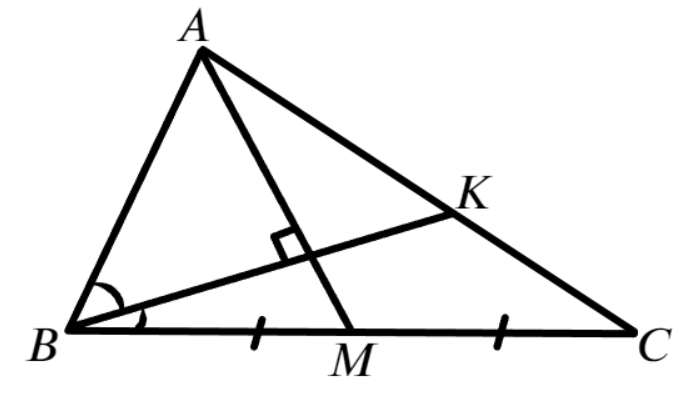
\includegraphics[scale=0.35]{g7-139.png}}
\end{figure}\\
В треугольнике $ABM$ биссектриса совпадает с высотой, значит он является равнобедренным и $AB=BM=\cfrac{1}{2}BC=\cfrac{1}{2}\cdot12=6.$\\
